\documentclass{article}
\usepackage{tikz}
\usepackage{amsmath}
\usepackage{lmodern}
\usepackage{xcolor}
\usetikzlibrary{calc}
\usetikzlibrary{decorations.markings}

\begin{document}

\centering

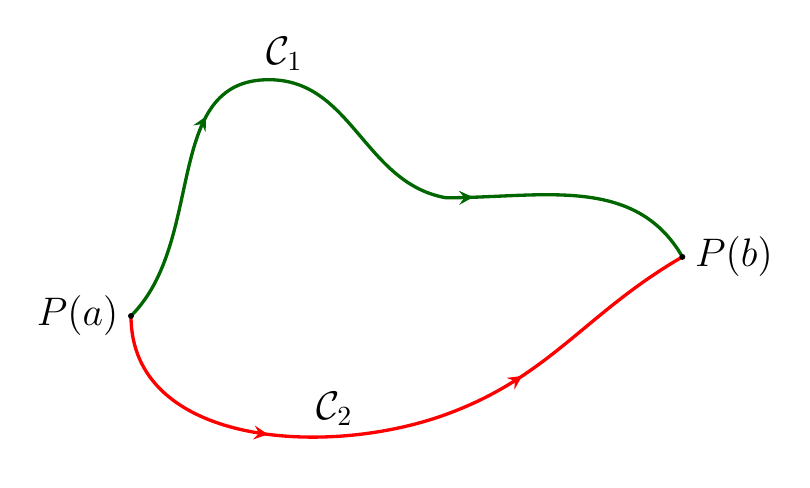
\begin{tikzpicture}[scale=2.5]
\pgfmathsetmacro{\CircleSize}{0.03}     % radius of coordinate circles/dots
% define styles used in this picture
\tikzset{every node/.style={font=\Large, text=black},
CircleNodeStyle/.style={draw=black, shape=circle, fill=black, minimum size=\CircleSize*2 cm, inner sep=0pt},
arrowstyle/.style={->, >=stealth}}

% custom colors
\definecolor{Green}{rgb}{0.0, 0.4, 0.0}
\definecolor{Red}{rgb}{1, 0, 0}

% defining smooth curve 1:
\coordinate (Begin) at (0.0, 0.0);
\coordinate (Bend) at ($(Begin)+(0.7, 1.2)$);
\coordinate (FlatMid) at ($(Bend)+(0.9, -0.6)$);
\coordinate (End) at ($(FlatMid) + (1.2, -0.3)$);
% decorate the path with marks along the path (markings must appear in ascending order along path!)
\draw[postaction={decorate}, decoration={
       markings,
       mark=at position 0.28 with {\arrow{stealth}},
       mark=at position 0.40 with {\node[above] {$\mathcal{C}_1$};},         % smooth curve symbol  
       mark=at position 0.7 with {\arrow{stealth}}}]
% draw the smooth curve
[very thick, Green] (Begin) to[out=45, in=180] (Bend) to[out=0, in=170] (FlatMid) to[out=0, in=120] (End);

% defining smooth curve 2:
\coordinate (Begin) at (0.0, 0.0);
\coordinate (Bend) at ($(Begin)+(1.6, -0.5)$);
\coordinate (End) at ($(Bend) + (1.2, 0.5+0.3)$);
% decorate the path with marks along the path
\draw[postaction={decorate}, decoration={
       markings,
       mark=at position 0.3 with {\arrow{stealth}},
       mark=at position 0.40 with {\node[above] {$\mathcal{C}_2$};},         % smooth curve symbol  
       mark=at position 0.7 with {\arrow{stealth}}}]
% draw the smooth curve
[very thick, Red] (Begin) to[out=270, in=200] (Bend) to[out=20, in=210] (End);

% corresponding dots with label after transformation
\node [CircleNodeStyle, label=left:$P(a)$] at (Begin) {};
\node [CircleNodeStyle, label=right:$P(b)$] at (End) {};

\end{tikzpicture}

\end{document}
